\documentclass[fleqn,10pt]{olplainarticle}
% Use option lineno for line numbers

\title{Dynamically created automations in Ambient Intelligence by using open-source automation software}

\author[1]{Peter Patočka {\tiny \href{ https://orcid.org/0000-0003-1468-8478}{\scshape 0000-0003-1468-8478}}}
\affil[1]{Department of Intelligent Systems, University of Technology, Brno, Czech Republic}

\keywords{Ambient Intelligence, Artificial Intelligence, Internet of Things, open-source automation software, smart home, Reinforcement learning, Home Assistant}

\begin{document}

\flushbottom
\maketitle
\thispagestyle{empty}

\vskip10pt

An ambient intelligent environment is an environment in the real-world, sensitive to human presence that reacts appropriately to human interactions. The term Ambient Intelligence (AmI) is relatively new. It was introduced by the Information Society Technologies Advisory Group in 2003 \cite{Istag2003}. This kind of environment gathers data from its surroundings using sensors and affects it by using actuators. Sensors and actuators, our intelligent agents, could be imagined as physical devices connected to the internet or intranet via various communication technologies, e.g. Wi-Fi, Bluetooth, RFID, Zigbee, or Z-Wave \cite{ElAzab2021}.

\vskip10pt

Ambient Intelligence is connected with Artificial Intelligence (AI), some even say that AmI is de facto AI in the environment \cite{Sukreep2020}. Big Data as the fuel for AI analyzes users’ actions, tries to predict their next steps, and creates automated rules or triggers to minimize user interactions with the systems. Users could be owners of the system who have control over the mechanisms or simple visitors with passive participation, but their presence is considered and taken into account either way. One of the biggest challenges in the field is the detection of human presence and human verification. Multiple sorts of sensors should be used to determine the exact position and state of the user.

\vskip10pt

AmI could be implemented in numerous application areas, including households, workplaces, elder care, schools, smart cities, or any other public places. For a lot of areas, it is probably safe to consider its position as supplementary to the existing process. The real value should be to ease routine, day-to-day activities and to enhance human-to-human interaction that should be replaced by human-to-system and finally human-to-environment interaction, without the necessity to interact with the system directly via a user interface.

\section{Related work}

Authors from the National University of Distance Education in Madrid \cite{Solano2017} created a custom implementation of vending machines, connected to the internet that allows cashless mobile NFC payments by using Arduino open-source hardware and software. Their main reason for not using Raspberry Pi is that Arduino is much simpler, without the need to load the whole operating system. Due to this fact, the system is much more stable and immune to power outages. OS should be properly shut down before turning ON and OFF.

\vskip10pt

Another example prototype of an Arduino-based vending machine with digital payment possibility is an innovative IoT platform \cite{Alam2021}. The backend of this mobile application was implemented in an open-source PHP framework Laravel.

\vskip10pt

Authors from the Department of Computer Science and Engineering created a smart parking management system (SPMS) with dynamic pricing based on the MCPR algorithm to search for and assign possible parking places \cite{Mondal2021}. Their solution allows the driver of vehicles to find and reserve the most appropriate parking space from anywhere at any time. As a consequence, it reduces traffic congestion, which reduces air pollution caused by unnecessary driving to find a proper parking area.

\vskip10pt

Andres Rico, Carson Smuts, and Kent Larson from MIT Media Lab in Cambridge used supervised (Recurrent Neural Networks composed of 8 layers) and unsupervised machine learning techniques (Spectral Clustering algorithm) to monitor activity and use of space in smart buildings \cite{Rico2022}. As they named it, the Chameleon system is composed of 3 main parts: the sensor board module, database in PostgreSQL, and Machine Intelligence Module which is enabled by the hybrid machine learning.

\vskip10pt

As an example of a system that uses open-source building automation software, I would mention the Secure Wireless Home Automation System implemented by a research group from Department of Computer Engineering in Ghana \cite{Sowah2020}. The system uses Open Home Automation Bus (OpenHAB 2) framework and they added an additional security layer by implementing JSON Web Token (JWT) interface and Advanced Encryption Standard (AES) procedures that support authentication and data encryption.

\vskip10pt

Base Cube One \cite{Pohling2019} is a location-addressable service-oriented smart environment framework connected to open-source building automation software. Connection is established via REST API and the system maps internal units and services into appropriate things/items in OpenHAB 2 software. Authors from Ambient Intelligence Group located in Bielefeld University also developed an augmented reality Android application named BComfy that allows 3D scans of rooms and other environments.

\section{The architecture system diagram}

In figure 1, there is a particular part of the Ambient Intelligent environment for registering \textbf{Internet of Things} (IoT) \cite{Atzori2010} devices to the building automation software (BAS) that supports creating automation rules or immediate manipulation with the IoT devices via some API, e.g. via REST.

\vskip10pt

In the diagram below, a central control unit (yellow), is connected to all IoT devices directly (green) through MQTT protocol and using various communication technologies, e.g. Wi-Fi, Zigbee, or Z-Wave. IoT devices could be integrated as a service (blue) indirectly with BAS by using a 3rd party API, e.g. Google Assistant, Amazon Alexa, or another BAS, such as openHAB. The central control unit behavior could be simulated without using real IoT devices. BAS simulator should provide the same communication interfaces as the real simulated unit.

\vskip10pt

The central part of the implemented architecture (orange) is Apache Kafka for stream data processing to multiple databases. We store structured, normalized data in the relational database (gray) as well as analytical data in the time series database. Normalized data in the relational database is ready for end-users to interact with the system via mobile application or website (light gray). Analytical data is available for AI algorithms to analyze user interaction within the system and predict users’ next steps. The system will take actions and automation rules based on this analysis.

\begin{figure}[ht]
    \centering
    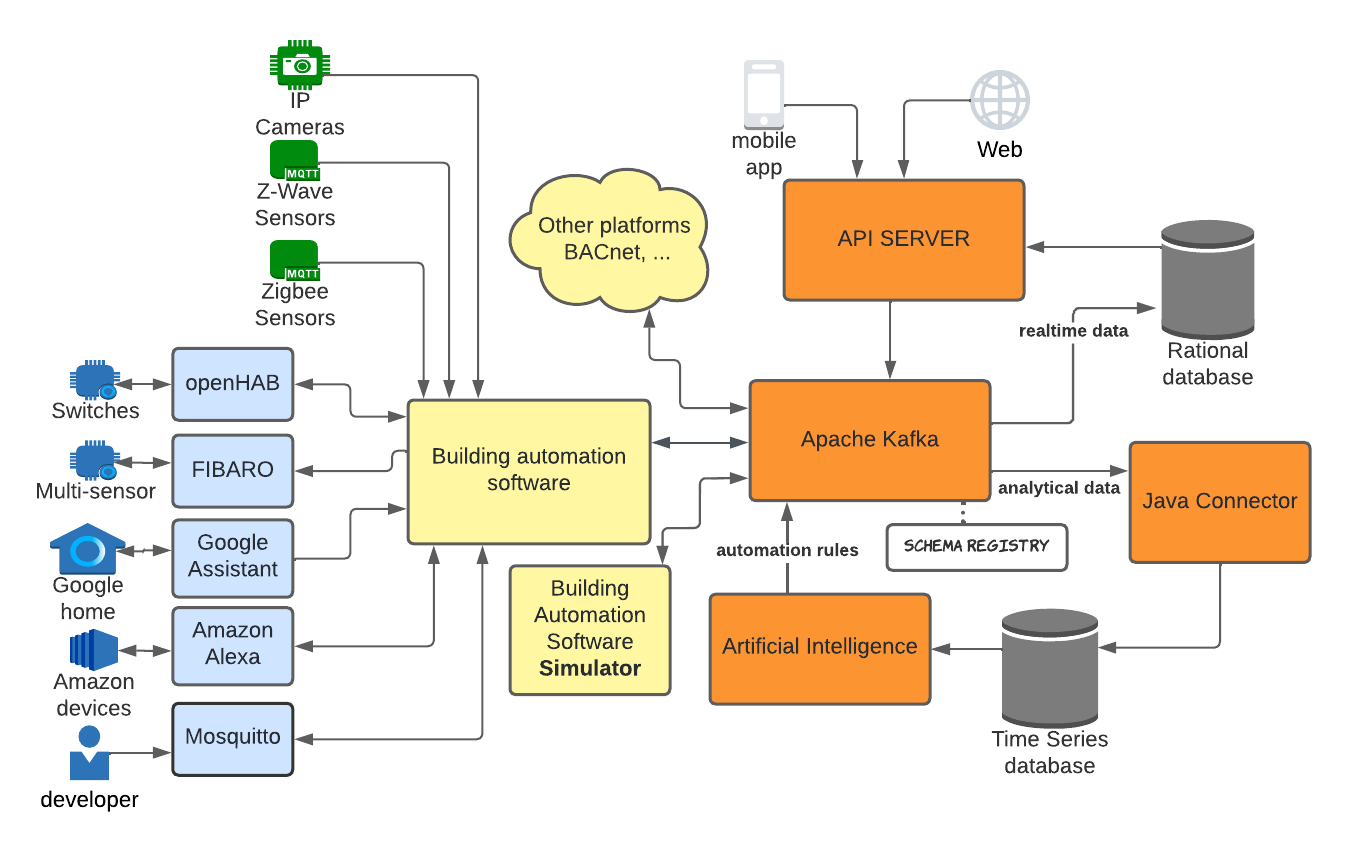
\includegraphics[width=1\linewidth]{images/IoT model big picture.png}
    \caption{Architecture of the desired system}
    \label{fig:figure1}
\end{figure}


\section{Open-source building automation software}

Building automation software (BAS) is designed to control the ambient intelligent environment via IoT devices that could control lighting, entertainment systems, home appliances, temperature, humidity, and purity of the air, together known as HVAC (Heating, ventilation, and air conditioning).

\vskip10pt

There are several attributes and features that BAS should support.

\vskip10pt

First of all, connectivity to IP (Wi-Fi, Bluetooth) and non-IP (ZigBee, Z-Wave) wireless communication technologies must be supported. Communication via IP protocols is naturally included in the system core since BAS is connected to the internet and all intranet devices are accessible. Non-IP communication technologies require using of an additional gateway. It could be in a form of a plug and play USB device that enables desired wireless communication type. A comparison of different types of communication technologies is described by M. Asadullah and A. Raza in \cite{Asadullah2016}. Another comparison based on power consumption, range, cost, and scalability was made by S. J. Danbatta and A. Varol in \cite{Danbatta2019}.

\vskip10pt

Due to the fact, that a lot of affordable devices are manageable exclusively through custom gateways of their manufacturers, interoperability, thus integration to 3rd party IoT services and platforms is another important aspect to track. Large manufacturers, like Google or Apple, support also voice assistants that could be used through integrations as well. However, direct support of voice activation is a welcomed feature offering independence of specific manufacturers and allowing to operate the voice assistant without interruption when external service is unavailable or deprecated.
Then, another important metric is the usability of the system. Starting with a simple and clear dashboard UI, BAS should provide a direct server API to control devices remotely. An example of remote control as such is MQTT, REST, or WebSocket. BAS should also allow the creation of automation scripts, triggers, and rules to automate actions without the necessity to interact with the software remotely.

\vskip10pt

Finally, considering AmI in public environments, BAS must emphasize security, operability, and stability. It should allow the making of backups and executing rollback if necessary. Moreover, it should support deployment to multiple architectures like Raspberry Pi or Docker Container. A custom operating system to watch over updates and monitor resources is also appreciated.

\vskip10pt

The most popular open-source BAS is listed in table \ref{tab:table1}.

\begin{table}[h]
\begin{tabular}{p{2.5cm} p{2cm} p{2cm} p{5cm}} \toprule
    Name & Core contributors & Primary language & Code repository URL  \\ \midrule
    openHAB & 104 & Java & https://github.com/openhab \\ \bottomrule
    Home Assistant & 2891 & Python & https://github.com/home-assistant \\ \bottomrule
    jeedom & 128 & PHP & https://github.com/jeedom \\ \bottomrule
    ioBroker & 160 & Javascript & https://github.com/ioBroker \\ \bottomrule
    openmotics & 15 & Python & https://github.com/openmotics \\ \bottomrule
    homebridge & 108 & Javascript & https://github.com/homebridge \\ \bottomrule

    openHAB & 104 & Java & https://github.com/openhab  \\ \bottomrule
    \end{tabular}
    \caption{\label{tab:table1}List of open-source home automation software}
    \end{table}

Some of them, like ioBroker and openHAB, are based on Eclipse SmartHome framework \cite{EclipseSmartHomeProject}, which offers a way to integrate smart home solutions with various protocols and standards, usable on any kind of system that can run an OSGi stack – multi-core server, a residential gateway or a Raspberry Pi. Unfortunately, this framework has been archived since May 2020.

\section{Selected build automation software - Home Assistant}

Home Assistant was introduced in September 2013 as a Python application by Paulus Schoutsen. It has the most contributors among all building automation open-source software. It has been listed in GitHub 2018 Octoverse project report in ninth place in the list “Fastest growing open-source projects” and in "State of the Octoverse" 2020 report in second place in the list “Top 10 Python packages with the most unique contributors over the last 12 months” \cite{GitHubStateOfTheOctoverse}. As it could be seen in figure \ref{fig:figure2}, the number of contributions is gradually increasing.

\begin{figure}[ht]
    \centering
    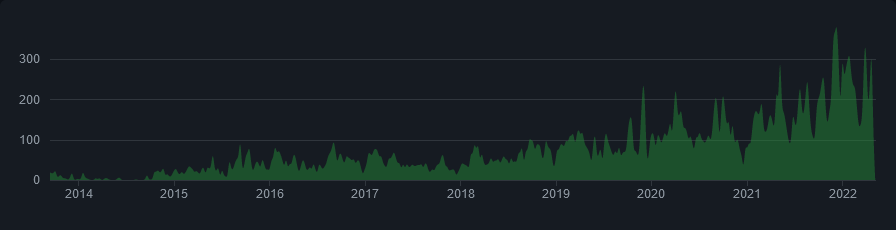
\includegraphics[width=1\linewidth]{images/contributors - hassio.png}
    \caption{Commit contributions to Home Assistant core project between Sep 15, 2013 – May 11, 2022 \cite{HassioContributors2013-2022}}
    \label{fig:figure2}
\end{figure}

Since Home Assistant is an open-source project, integrations to 3rd party services are provided by the community. Currently, over 1970 integrations are supported, including Google Assistant, Amazon Alexa, Apple iCloud, Apache Kafka, and InfluxDB.

\vskip10pt

Smart home automation software should detect new IoT devices and support a simple and unified way to add and remove various devices automatically.

\subsection{Auto-configuration}

Automatic device discovery is usually included in protocols Devices Profile for Web Services (DPWS) and Universal Plug and Play (UPnP). Unfortunately, some IoT devices, like Arduino, do not support DPWS. One possible solution to this issue is to include a Device Manager that detects new devices via MQTT protocol directly in IoT Home Gateway. MQTT handles connections also with non-IP devices (Zigbee, Z-Wave, Bluetooth). The solution is pictured in figure \ref{fig:figure3}.

\begin{figure}[ht]
    \centering
    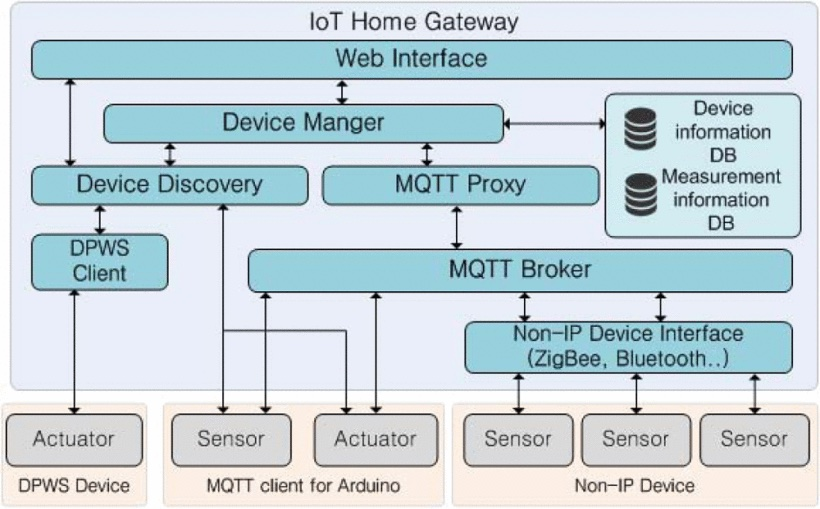
\includegraphics[width=1\linewidth]{images/device manager.jpg}
    \caption{Device manager and MQTT Proxy in IoT Home Gateway. Source: \cite{Kim2015}}
    \label{fig:figure3}
\end{figure}

A feature that allows registering and unregistering devices ad-hoc without the necessity to change configuration properties manually is called auto-configuration. It should work regardless of communication protocol, architecture type, or brand.

\vskip10pt

In Home Assistant, MQTT Discovery is enabled by default.

\subsection{Architecture and maintenance}

Home Assistant runtime package consists of \textbf{core} and operating system \textbf{supervisor}. There are several installation methods available. Whereas core developers are encouraged to run core directly in Python virtual environment, recommended deployment is within a bundle of a custom operating system for Raspberry Pi, ODROID, ASUS Tinkerboard or Generic x86-64 UEFI device. Virtualization in Windows, MacOS, and Linux is also supported. Home Assistant core is also possible to start in a Docker container.

\vskip10pt

The whole runtime package could be automatically updated in configuration UI or via the CLI command \mintinline{shell}{ha core update -version 2022.5.4} where \mintinline{shell}{-version} is an optional parameter and if it is omitted, then the latest version is downloaded.

\vskip10pt

Before updating, it is recommended to search in release notes for breaking changes and do a system backup. As usual, \textbf{full or partial backups} could be made from UI, command-line interface, or created automatically by using a custom Blueprint (which is not part of the basic installation). Since backups are compressed to a single .tar file, it is endorsed to copy the archive to an external directory or cloud service.

\vskip10pt

\textbf{Blueprints} are reusable code blocks created and shared by the community to be called with different parameters.


\subsection{Configuration}

Despite the fact that every configuration could be handled via dashboard UI, at the end of the day, all configurations are stored in YAML files. YAML is a human-readable data serialization language \cite{YamlSpecification122} with an indentation style very similar to the Python programming language.

\vskip10pt

The main configuration file is configuration.yml and it supports nesting by importing files with the command \mintinline{shell}{!include filename.yml}, respectively by importing the content of directories with the commands \mintinline{shell}{!include_dir_list}, \mintinline{shell}{!include_dir_named}, \mintinline{shell}{!include_dir_merge_list}, or \mintinline{shell}{!include_dir_merge_named}.

\vskip10pt

By default, overwriting YAML files remotely is not supported. However, there are multiple add-ons available that enable remote connection, like Samba share, Terminal \& SSH or simple File Editor. Configuration needs to be reloaded when it is updated remotely. All configurations are reloaded after a restart, although some configurations can reload via dashboard UI without requiring a restart, e.g. Automations, Groups, People, Scenes, Scripts, Timers, and Zones.

\vskip10pt

When the configuration file is changed, it is recommended to check if the configuration is valid by using a validation tool in Developer Tools or by the command in ssh \mintinline{shell}{ha core check}.

\subsection{Automations}

A way to define automatically executed actions is via automation scripts. They could be defined from the dashboard UI or directly in YAML files. Automations are basically actions triggered by some event and executed when a condition is satisfied. There is no limitation to the event types and some of them are included in the default built-in library.

\vskip10pt

Some of the most common event types are:

\vskip10pt

\begin{itemize}
    \item $call\_service$ is fired when a service is called
    \item $automation\_triggered$ is fired when an automation script is triggered
    \item $homeassistant\_started$ is fired after Home Assistant startup (after a reboot)
    \item $state\_change$ is fired when an entity state is changed
\end{itemize}

A trigger is a hook that invokes automation. A single automation script could have multiple triggers. A condition is an optional part of the rule. It uses the system’s current state to check the validity of the statement. By contrast, the trigger does not look at the system state and reads data from events invoked in the environment. Besides the input source, a logical relation between triggers is OR. It means that if any of the defined triggers are invoked, conditions are validated and if the final composed condition is satisfied, then action is executed. The default logical relation between conditions is AND. However, OR, NOT, and a mix of all logical relations could be used too.

\vskip10pt

There are some examples of conditions:

\begin{itemize}
    \item \textbf{State} – tests if the entity state is at the desired value. It is possible to pass multiple entities to test them at once.
    \item \textbf{Sun} – tests if the sun is above or below the horizon. Also, it is possible to define a positive or a negative offset.
    \item \textbf{Time} – tests if time is after or before at the specified range. A particular day of the week could be considered as well.
    \item \textbf{Template} – tests the template expression output to be true boolean or “true” string value. The template is a text processing feature used for data extraction and transformation, powered by the Jinja2 Python template engine.
\end{itemize}

\vskip10pt

It is noteworthy that automations use Blueprints defined in the YAML structure. A single Blueprint could be used multiple times in different automation scripts.


\subsubsection{Example automation}

To illustrate how automations are created we will define a simple automation script that will be

\begin{center}
    \textbf{turning on the light when a movement is detected in a dark hall.}
\end{center}

\noindent Such a sentence could be transformed into a sequence of triggers, conditions, and actions:


\begin{table}[h]
\begin{tabular}{p{3cm} p{10cm}} \toprule
    \textbf{Trigger} & Motion sensor detects movement in the hall.\\ \bottomrule
    \textbf{Condition} & The hall light is below 20 lux.\\ \bottomrule
    \textbf{Action} & Turn on the light in the hall.\\ \bottomrule
    \end{tabular}
    \caption{\label{tab:table2}Turning the light on movement in the hall when the hall light is below 20 lux}
    \end{table}

When the sentence is transformed into a set of rules, we could write the automation in YAML format and store it into file \textbf{automations.yml}.

\lstinputlisting[caption=Automation rule in \textit{automations.yml}]{code/automations.yml}


\subsection{REST API}

REST API serves as a real-time communication between Home Assistant and any external system. A new "Long-Lived Access Token" needs to be generated in the user’s profile and included in every HTTP operation to authorize every HTTP request.
Server returns HTTP status 200 (OK) or 201 (Created) on success. Otherwise, a 400 (Bad Request), 401 (Unathorized), 404 (Not Found), or 405 (Method Not Allowed) is returned.

\vskip10pt

There are several important endpoints to determine current state and to control devices registered in a Home Assistant network. First of all, to ensure the REST API is working, we could hit GET \mintinline{shell}{/api/} that returns a constant message “API running” with status 200 (OK) if everything is working well. Endpoint GET \mintinline{shell}{/api/states/} returns all state objects. State object contains entity\_id, state, last\_changed and attributes. Similarly, another endpoint GET \mintinline{shell}{/api/services/} returns all service objects. A single service object contains domain name and a list of services.

\vskip10pt

In order to control devices in the network, the service POST \mintinline{shell}{/api/states/${ENTITY_ID}} is not exactly what to look for. This endpoint just updates a simple state. It will not reach the actual device. To communicate with the existing device in the network and change its internal state and do appropriate action, use POST \mintinline{shell}{/api/services/${DOMAIN}/${SERVICE}}. Request JSON body is optional here, but it is used to define an entity to operate with. A JSON string is returned with a list of changed states during the endpoint being executed. A working example is in listing \ref{code:listing2}.

\lstinputlisting[caption=\label{code:listing2}Turn on wall\_switch light via REST API \cite{RestApiDocumentation}]{code/rest_api_turn_on_switch.txt}

\section{Reinforcement Learning}

Reinforcement learning (RL) is one of the machine learning categories, somehow similar and related to supervised and unsupervised machine learning, although with different approach to the learning process.

\vskip10pt

Supervised machine learning algorithms are learning from a large set of data labeled by a supervisor. Labeled data are augmented by the set of training samples to verify that the supervised algorithm has learnt a correct model. Whereas supervised learning is overseen by a machine learning specialist that labels training data. Unsupervised learning does not have data labeled.

\vskip10pt

There is also a combination of both supervised and unsupervised learning, named Semi-supervised learning, where learning algorithms receive a small set of labeled, as well as a large set of unlabeled training data. Then it learns from labeled data and applies what it has been learnt to make some predictions to unlabeled data \cite{Chapelle2010-mm}.

\vskip10pt

RL is similar to Semi-supervised learning. Usually, it is quite supervised and has labeled and unlabeled data available as well. Nonetheless, the approach is incremental and instead of learning from a large volume of data. It is more a trial-and-error behavior, where an agent does some pseudo-random action, looks at the reward, and evaluates it. Next steps are taken in order to maximize reward and minimize punishment. It is worth mentioning that actions should also consider subsequent rewards, not only immediate ones.

\begin{figure}[ht]
    \centering
    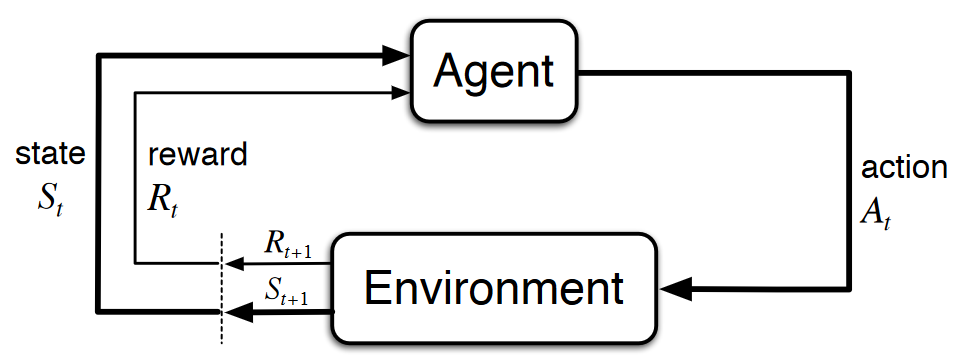
\includegraphics[width=0.7\linewidth]{images/reinforcement_learning.png}
    \caption{Reinforcement algorithm. Source: \cite{Sutton1998-ta}}
    \label{fig:figure4}
\end{figure}

Let’s look at some reasons why RL is the right machine learning category for an Ambient Intelligent environment.

\vskip10pt

Firstly, most machine learning categories see the world as a constant place and any possible change in the environment will invalidate their results. As we know, AmI is quite a dynamic environment. Thanks to auto-configuration our IoT devices (sensors and actuators) are registering and unregistering constantly at any moment. They could also adjust their position in the environment, thus they could change their assignment into rooms as well as be temporarily displaced and moved back again. Disabling devices, as well as turning them off due to the dead battery, is something that should be considered in RL too.

\vskip10pt

Secondly, supervised and unsupervised learning categories do not work very well with modifying goals. Consider the following situations: a new person comes to live in a smart house, a company reorganizes its infrastructure, or the whole production hall is bought by another corporation. Those are new subjects with various requirements for the environment. An environment's behavior needs to fit better with these new requirements.

\vskip10pt

Finally, RL does not require enormous time to learn. Instead of that, it takes immediate actions and observes outcomes. Then it calculates rewards and punishments and reacts to the new situation. Besides that, RL does not differ so much in rapidly expanding systems.

\subsection{Formalization}

RL could be formalized as \textbf{Markov Decision Process}, represented by a tuple

$$M = \langle S, A, P, R, \gamma \rangle$$

\noindent where

\begin{itemize}
\item $S$ is the set of states
$$s \in S$$
\item $A$ is the set of actions
$$a \in A$$
\item $P$ is the transition probability function, which defines a probability of taking an action $a$ in a state $s$ leading to the new state $s'$
$$p : S \times S \times A \in [0,1]$$
$$p(s' \mid s,a) \doteq P\{S_t = s'\mid S_{t-1} = s, A_{t-1} = a\} $$
\begin{center}
$\sum_{s' \in S} p(s' \mid s,a) = 1$, for all $s \in S, a \in A(s)$
\end{center}
\item $R$ is the reward function, which predicts the next reward $r$ from taking action $a$ from state $s$
$$r : S \times A$$
\item $\gamma$ is the discount factor, which determines the present value of future rewards.
$$\gamma \in [0,1]$$
The more closer the $\gamma$ value is to 1, the more seriously takes algorithm into account future rewards.
\end{itemize}

Environment is considered as a discrete, hence time independent, where each time step $t = [0,  \infty)$ is represented by the state $S_t \in S$. When some action is taken $A_t \in A$, one step later agent receives numerical reward $R_{t+1} \in R$. This is called immediate reward, when a reward is received one step after action is executed. During evaluation of the state, there are also future rewards considered, defined as $R_{t+k}$ for $k > 1$.

\vskip10pt

To evaluate the current state, the sum of all future discounted rewards is defined as the \textbf{return} ($G_t$), calculated by a formula:
$$G_t = \sum_{k=0}^{\infty} \gamma^k R_{t+k+1}$$

RL defined two important value function. The first is the \textbf{state value function} $v_{\pi}(s)$, that determines how good is for an agent to stay in a state $s$, which is represented by the sum of the future rewards:
\begin{center}
$v_{\pi}(s) = E_{\pi}[\sum_{k=0}^{\infty} \gamma^k R_{t+k+1} \mid S_{t}=s]$, for all $s \in S$
\end{center}

The second is the \textbf{state-action value function} $q_{\pi}(s,a)$, that determines how good is for an agent to stay in a state $s$ and taking an action $a$:
\begin{center}
$q_{\pi}(q,a) = E_{\pi}[\sum_{k=0}^{\infty} \gamma^k R_{t+k+1} \mid S_{t}=s, A_{t}=a]$, for all $s \in S$
\end{center}

State value function and state-action value function are following the \textbf{policy} $\pi(a \mid s)$, that decides which action $a$ should be taken, consider the current state $s$.

\vskip10pt

The goal of RL is to find the right policy to maximize a reward over a longer time period. Policy with the greatest return for all states is called \textbf{optimal policy} $\pi_{*}$. Optimal policy has the \textbf{optimal state value function} $v_{*}$, defined as:
\begin{center}
$v_{*}(s) \doteq \max_{\pi} v_{\pi}(s)$, for all $s \in S$
\end{center}

To decompose an optimal state-action value function into the immediate reward and discounted future values, we can use Bellman Optimality Equations \cite{AZUATALAM2020100020}.

\vskip10pt

Nowadays, a lot of research papers use RL \cite{Deng2021} and Deep Reinforcement learning (DRL) \cite{Brandi2020,McKee2020,Qin2021,Yu2020} algorithms, like SARSA, Q-learning, Deep Q-learning, and Actor–critic in IoT systems \cite{Frikha2021}.


\section{Conclusion}

In this document, I described the architecture of an Ambient Intelligent environment that allows us to create automations by using an open-source building automation software called Home Assistant, fueled by RL.

\vskip10pt

My proposed system writes all environment state changes to the time series database (InfluxDB), where they are available to machine learning algorithms. These take actions, generate automation rules, and interact with the environment directly via REST API.

\vskip10pt

One of the possible uses of the solution as such could be in HVAC management. Let’s consider an ideal temperature for users in an environment that will be set automatically, without the necessity to interact with control mechanisms. In the first place, the user has to be detected and recognized. Their movement and activity are observed and based on their previous interactions, the ideal temperature in the room is set up. Any interactions with HVAC controlling mechanisms are noted and penalized with an aim to minimize the user’s manual interactions with the system. Moreover, when the user changes position or activity, or a new person comes into the room, a new temperature should be set up to suit the new state of the environment.

\vskip10pt

The presented algorithm could be applied to other IoT categories, for instance, light control, security, entertainment systems, home appliances, humidity control, and others.

\vskip10pt\vskip10pt\vskip10pt

\pagebreak

\bibliography{bibliography}

\end{document}